%==================================================
%% chapter03.tex for NWPU Bachelor Thesis
%% Encoding: UTF-8
%%==================================================

\chapter{实验与结果}
\label{chap:Results}
本FAT32文件系统接口的整体编译并导出HEX文件后,约占据16KB的代码空间,该模块运行时所需内存空间至少(512B + 100B),其中「512B」是缓冲池大小,
「100B」是各模块的全局变量总大小。然而在进行实验验证时,还需为需要读写文件操作另行开辟一块内存空间(512B),故实际所需内存空间至少为「1124B」。
同时为了实验的便利性,简化不必要的操作,使单片机与SD卡在SPI模式下通信,又为了尽可能提高读写速度,最好使用硬件SPI接口。
结合以上需求,本实验最终选择了C8051F020芯片,其有「4352B」的RAM,「64KB」的FLASH,并且带有一个硬件SPI接口,完全符合要求。

\section{工作区的文件组成}
\label{sec:Workspace}
考虑到本文件接口的模块化设计和实现,在实验验证过程也将分模块进行实验。
当对FAT文件系统模块进行实验时,底层的「disk.c」和「disk.h」将被测试用的测试文件「fattest.c」和「fattest.h」代替。
工作区文件构成如图\ref{fig:wsp1}。

\begin{figure}[!htbp]
    \centering
    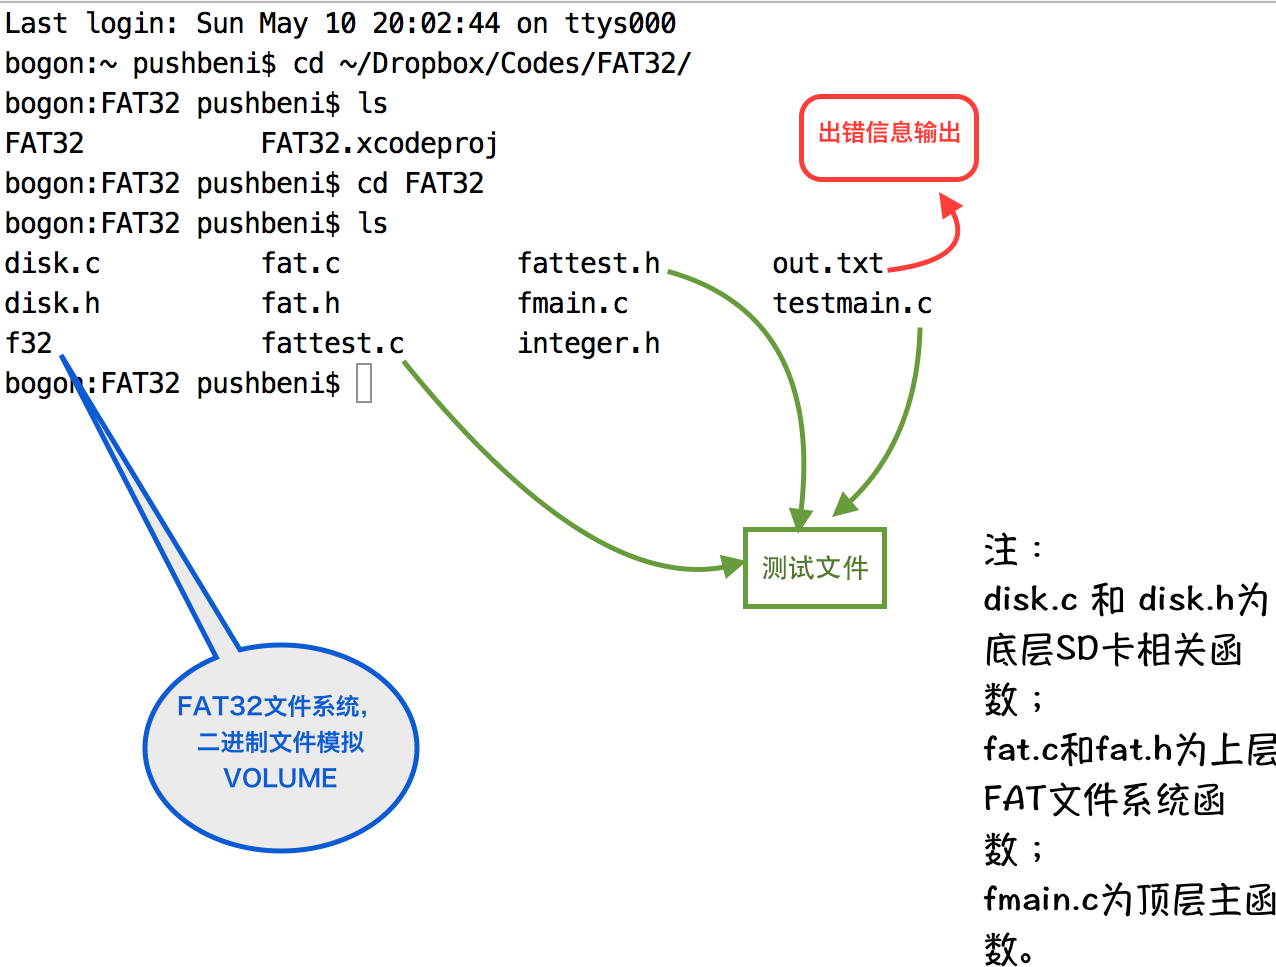
\includegraphics[width=1.0\linewidth]{chap4/workspace.png}
    \\
    \caption{工作空间} \label{fig:wsp1}
\end{figure}

其中的「f32」是一个二进制文件,用来模拟一个磁盘卷,以测试FAT模块的各项功能能否正确实现。「out.txt」是用来记录在FAT模块的各个函数换回值,
不仅用来记录出错信息,当FAT模块从“磁盘卷”(即「f32」文件)读出一个文件的数据后,测试程序会将读出的数据保存在这里供之后比对。
「testmain.c」就是在测试时的主程序,而「fmain.c」实际上就是「main.c」文件,是实际验证时的主程序文件。

当需要将两个模块组合在一起再次进行实际的实验时,
工作区的文件也要相应发送变化,之前的「fattest.c」和「fattest.h」将被真正的硬件层驱动函数「disk.c」所替换。
同时主文件也变成了「main.c」。
最终的工作区文件见图\ref{fig:wsp2}。
可以看到,本实验采用KEIL-C51进行源文件的编译并最终生成HEX文件烧如单片机,用C8051F的Debugger进行调试。

\begin{figure}[!htbp]
    \centering
    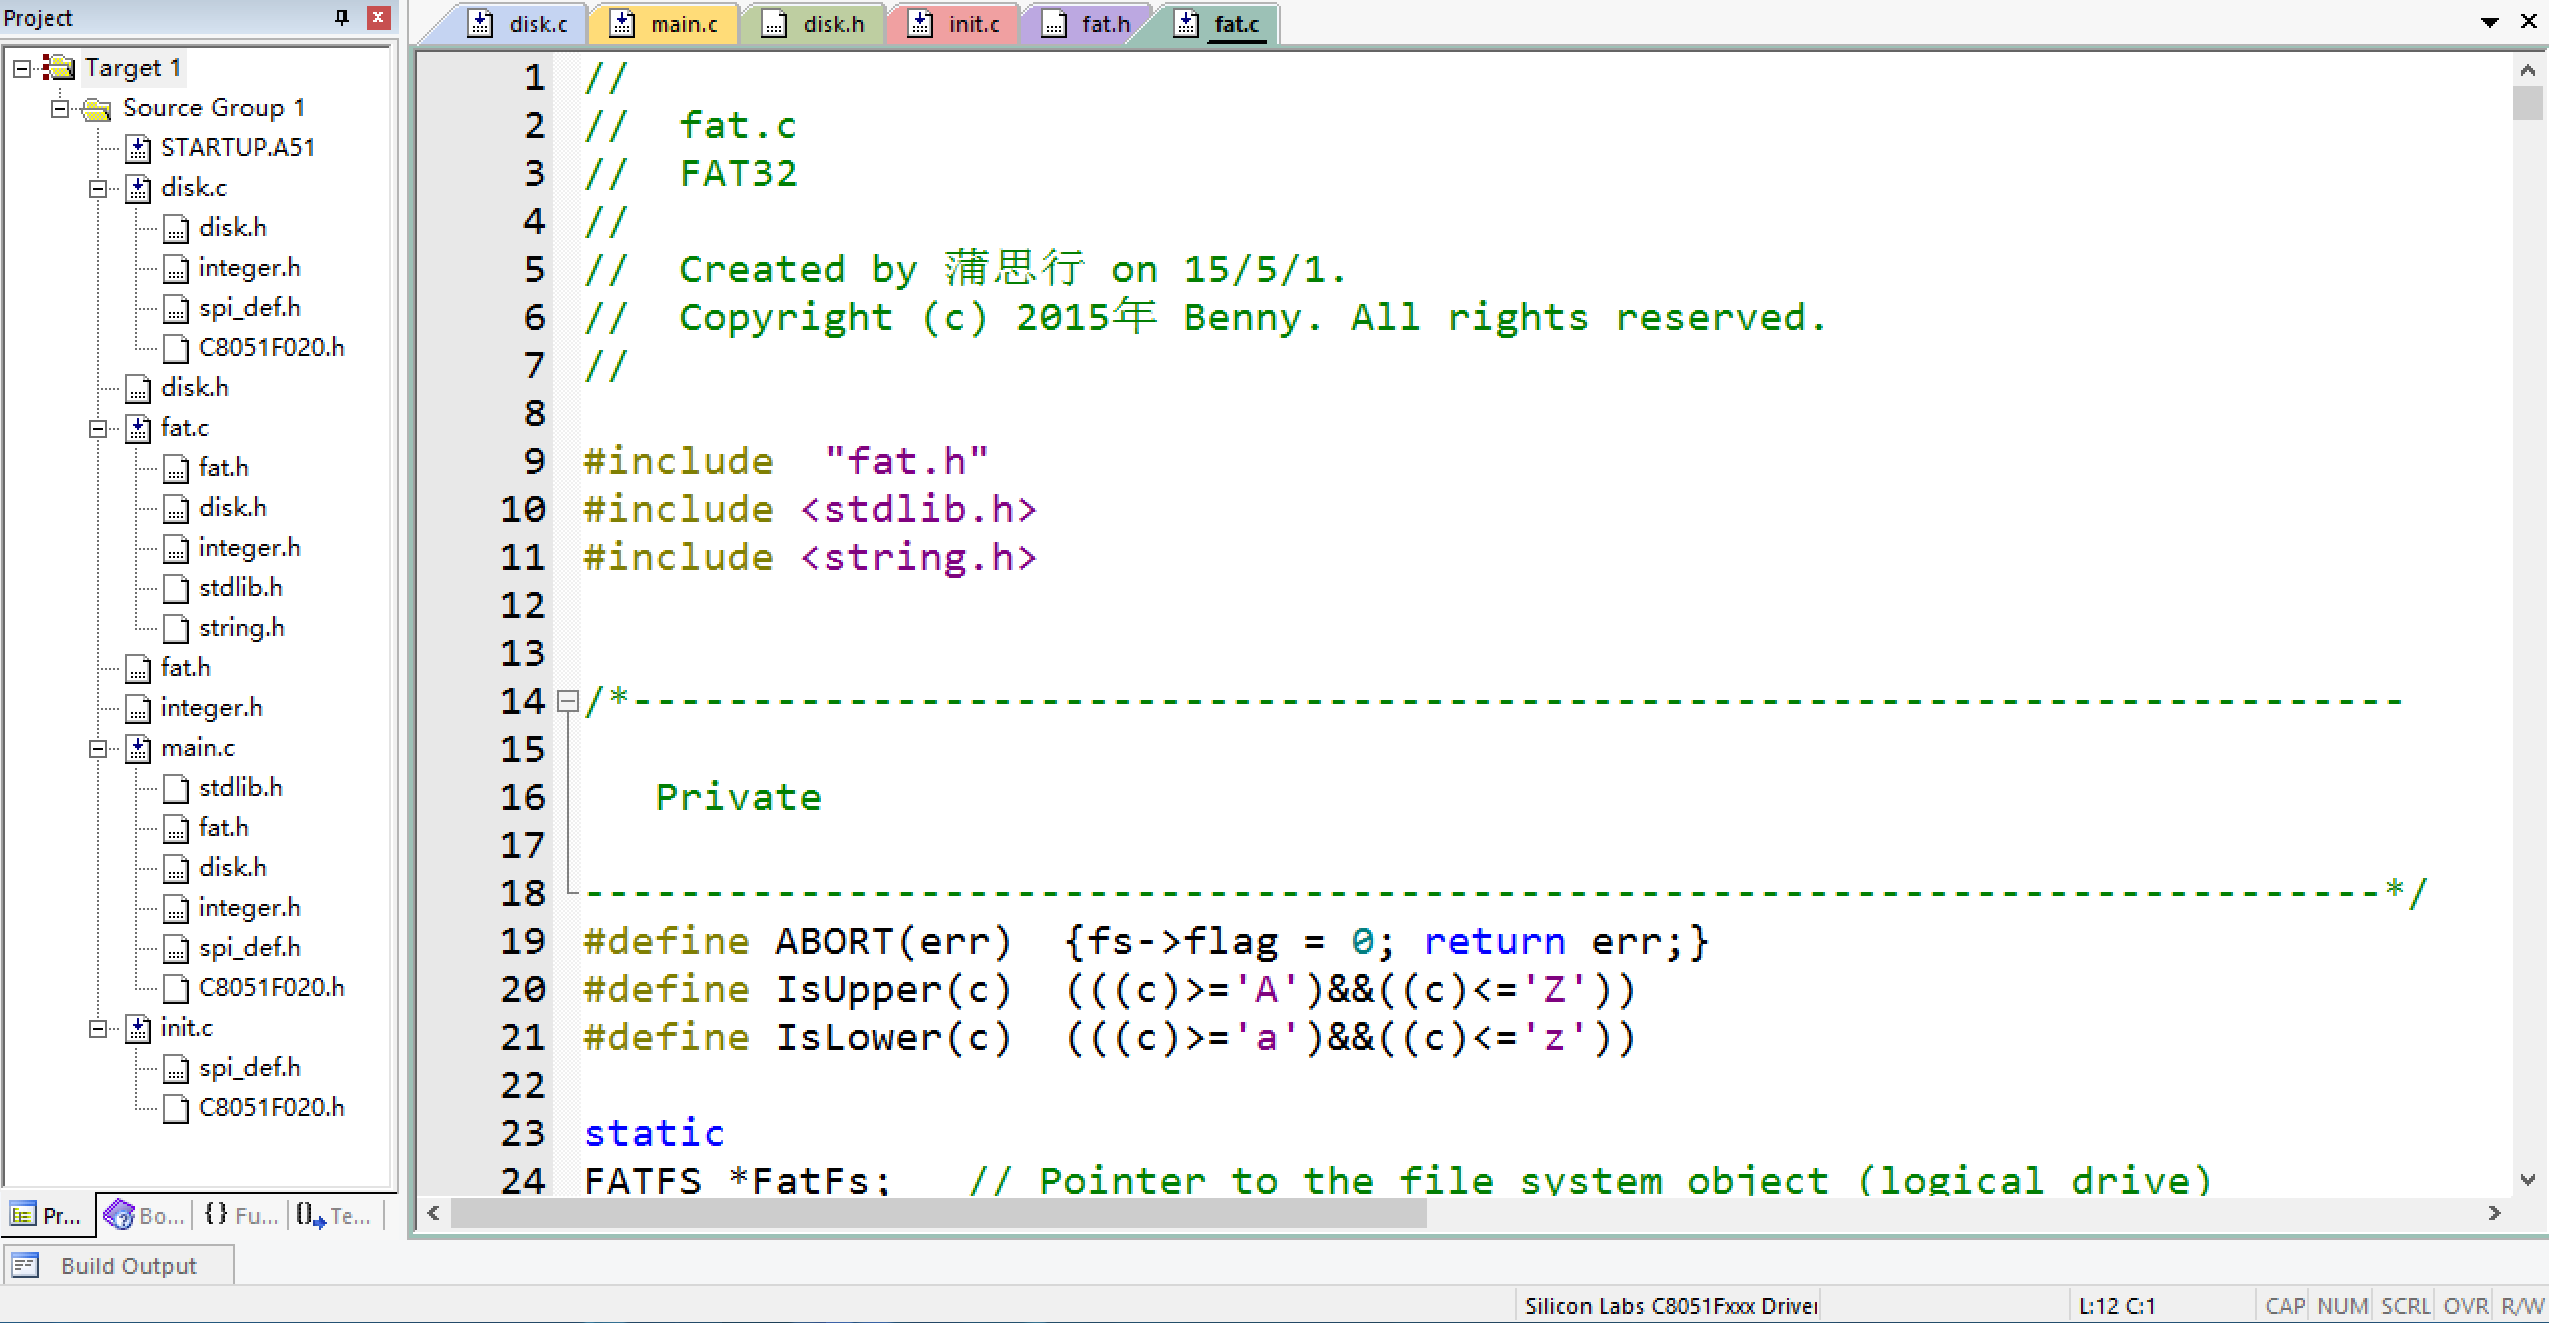
\includegraphics[width=1.0\linewidth]{chap4/workspace2.png}
    \\
    \caption{最终的工作空间} \label{fig:wsp2}
\end{figure}

\section{文件系统模块的逻辑验证}
\label{sec:ExpFAT}
文件系统模块的实验中,工作区如图\ref{fig:wsp1}。在这部分实验中,不需要考虑底层的情况,只需要相应函数功能在逻辑上能够正确无误的达成即可。
因此,为了模拟文件系统模块对物理磁盘的操作,实验时在磁盘上建立了一个无格式的二进制文件「f32」,用来模拟一个磁盘卷。当然,相应地,
测试文件「fattest.c」中的「disk\_\textit{xxx()}」之类的函数全部是通过「fopen()」、
「fread()」和「fwrite()」等函数\footnote{此处的「fopen()」等函数是在<stdio.h>中原生定义好的函数,用来实现对文件的操作,
不要与本文件接口定义的「f\_open()」等函数混淆}对文件进行操作。
但是在文件系统模块看来,好像是在对磁盘进行操作一样。

为了用「f32」二进制文件真正地模拟磁盘卷,首先要对它进行初始化配置,即将其“$0^{th}$”扇区(起始的512个字节)按照「DBR」启动扇区的格式填入正确的内容,
还要在“$1^{st}$”扇区按照正确的格式填入FSINFO扇区的内容。
配置好的「f32」文件如图\ref{fig:GUI}。

\begin{figure}[!htbp]
    \centering
    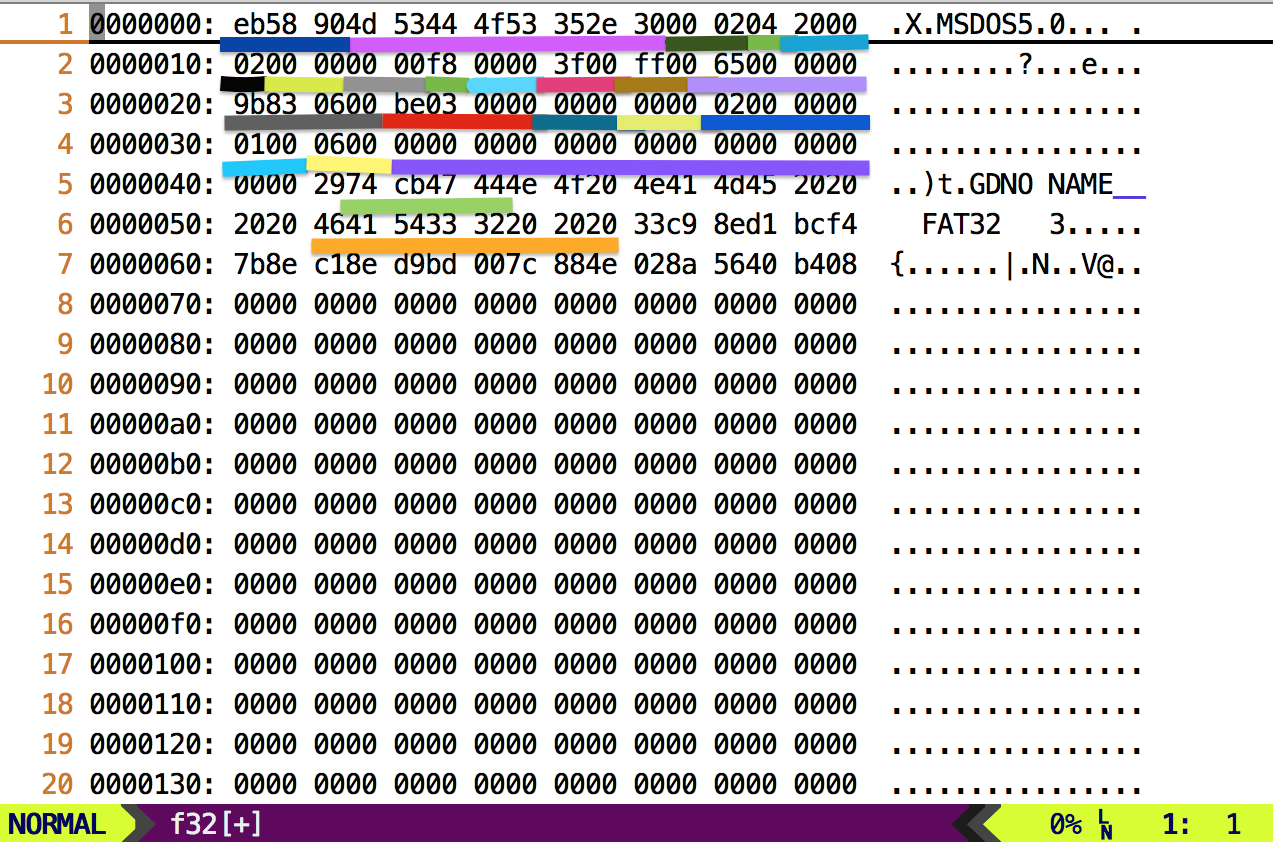
\includegraphics[width=1.0\linewidth]{chap4/GUI.png}
    \\
    \caption{模拟的启动扇区} \label{fig:GUI}
\end{figure}

文件系统挂载后,各项参数信息如图\ref{fig:mount}。
通过右下角的「lldb」调试信息可以看到,$*fs$的各项信息已经有了正确的值,并且从「res=FR\_OK」也知道了磁盘卷已经正确挂载。
可以看到,测试用的模拟的磁盘卷的簇大小为4个扇区,即2KB,「fs\_type」为「0x33」表是该文件系统是FAT32,
「fatbase」为「32」表示FAT表的起始扇区是32号扇区,即第「0x4000」字节处。「dirbase」为「2」表示根目录起始簇为2号簇,即第「0xF3800」字节处。

\begin{figure}[!htbp]
    \centering
    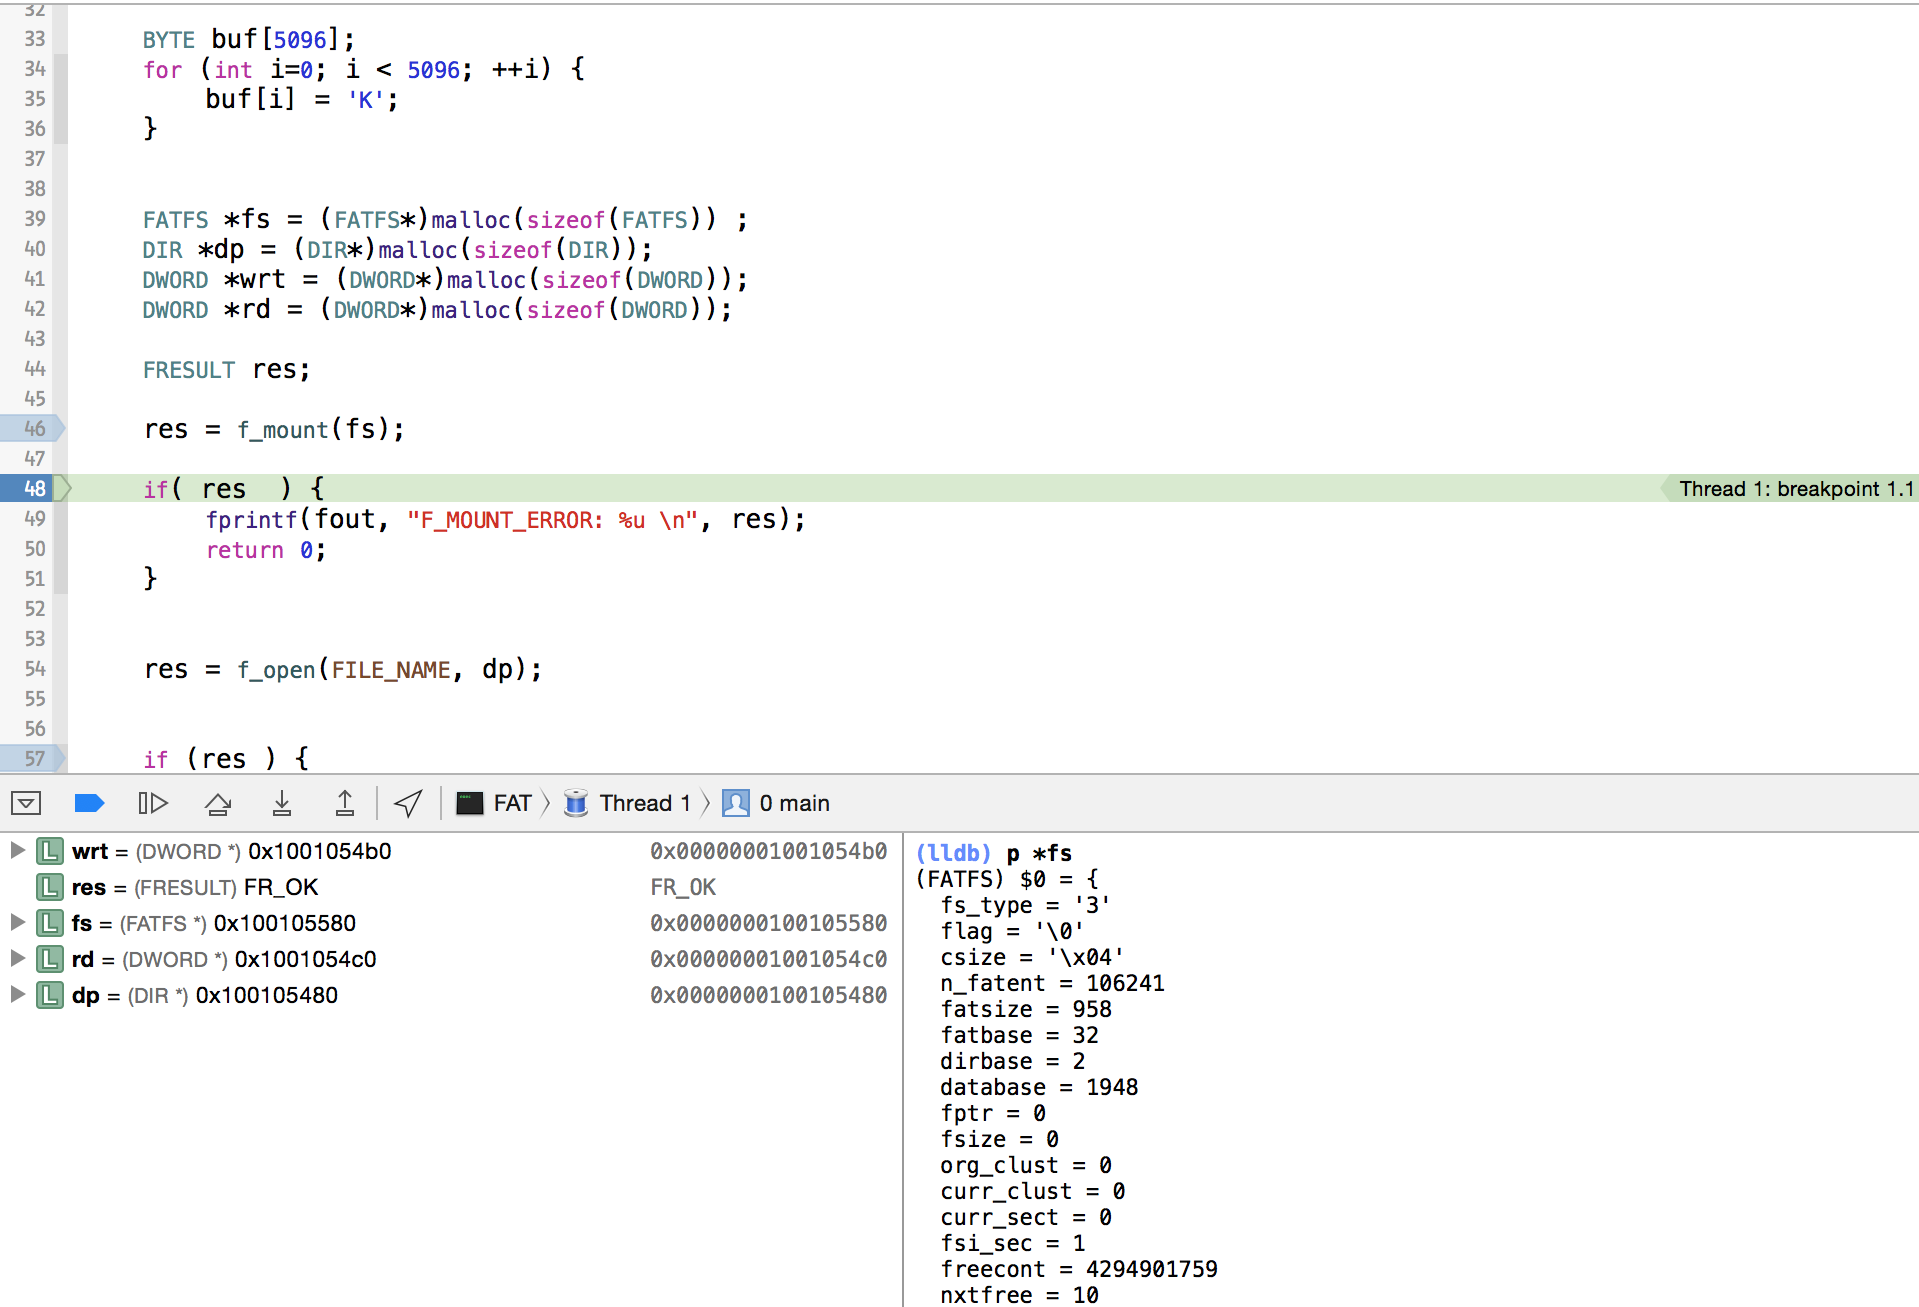
\includegraphics[width=1.0\linewidth]{chap4/mount.png}
    \\
    \caption{挂载文件系统} \label{fig:mount}
\end{figure}

接下来可以在根目录新建一些文件「TEXT1.TXT」、「TEXT2.TXT」和「TEXT3.TXT」,
新建文件操作后结果如图\ref{fig:dircrt}。

\begin{figure}[!htbp]
    \centering
    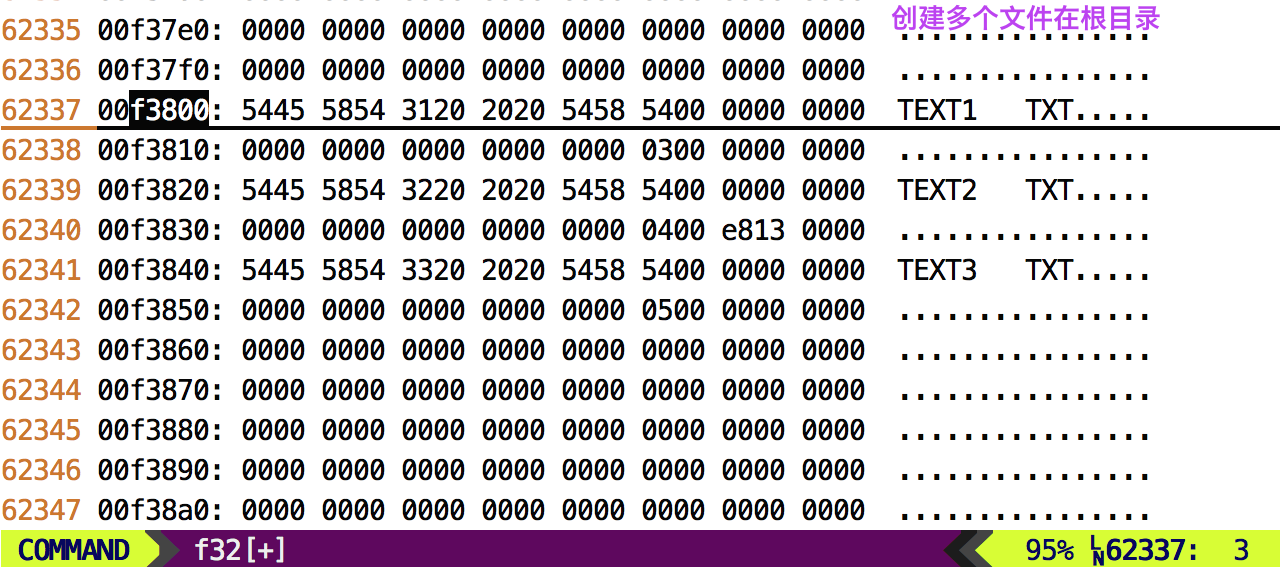
\includegraphics[width=1.0\linewidth]{chap4/dircrt.png}
    \\
    \caption{目录表中新建目录项} \label{fig:dircrt}
\end{figure}

之后进行写操作,写入超过一簇(如5096个字节)的数据后,FAT表会更新并续接簇链,写入后更新的FAT表如图\ref{fig:fatcrt}。

\begin{figure}[!htbp]
    \centering
    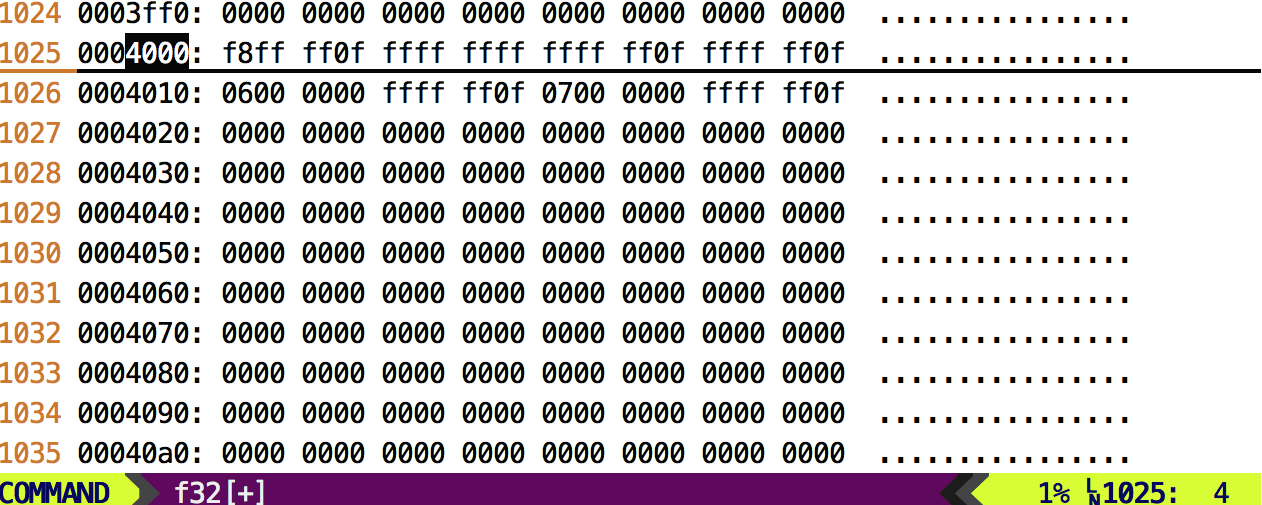
\includegraphics[width=1.0\linewidth]{chap4/fatcrt.png}
    \\
    \caption{FAT表分配新的簇号} \label{fig:fatcrt}
\end{figure}

写入数据后,磁盘卷的数据区如图\ref{fig:datawrt}

\begin{figure}[!htbp]
    \centering
    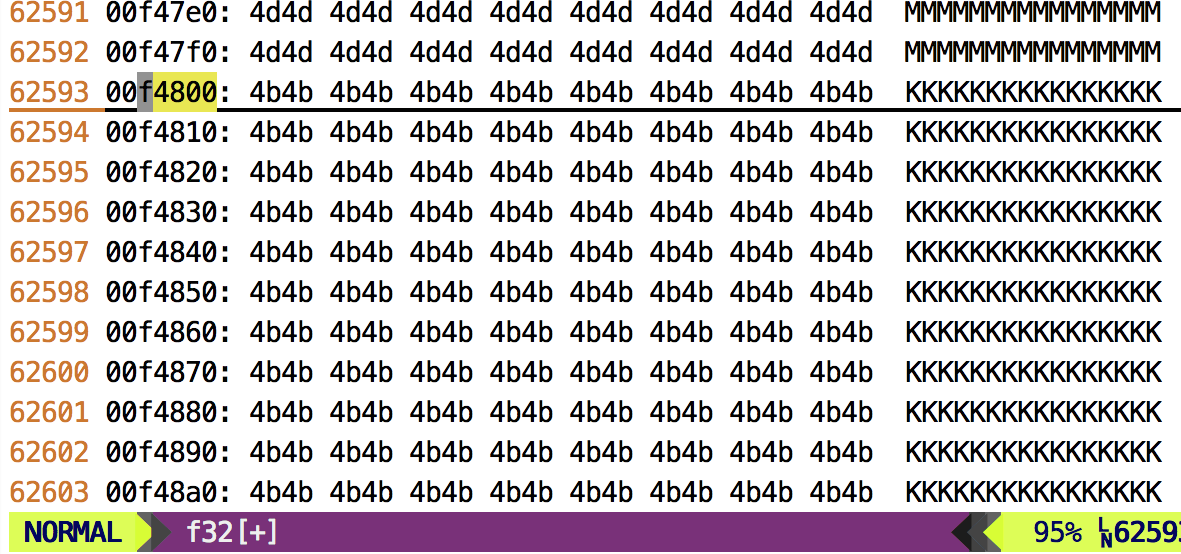
\includegraphics[width=1.0\linewidth]{chap4/datawrt.png}
    \\
    \caption{写入后的磁盘卷数据区} \label{fig:datawrt}
\end{figure}

当成功写入文件后,还要再测试从文件读取数据的过程,正确读取后返回值应为「FR\_OK」,同时缓冲池「buf」中应该有正确的数据,结果如图\ref{fig:datard}。

\begin{figure}[!htbp]
    \centering
    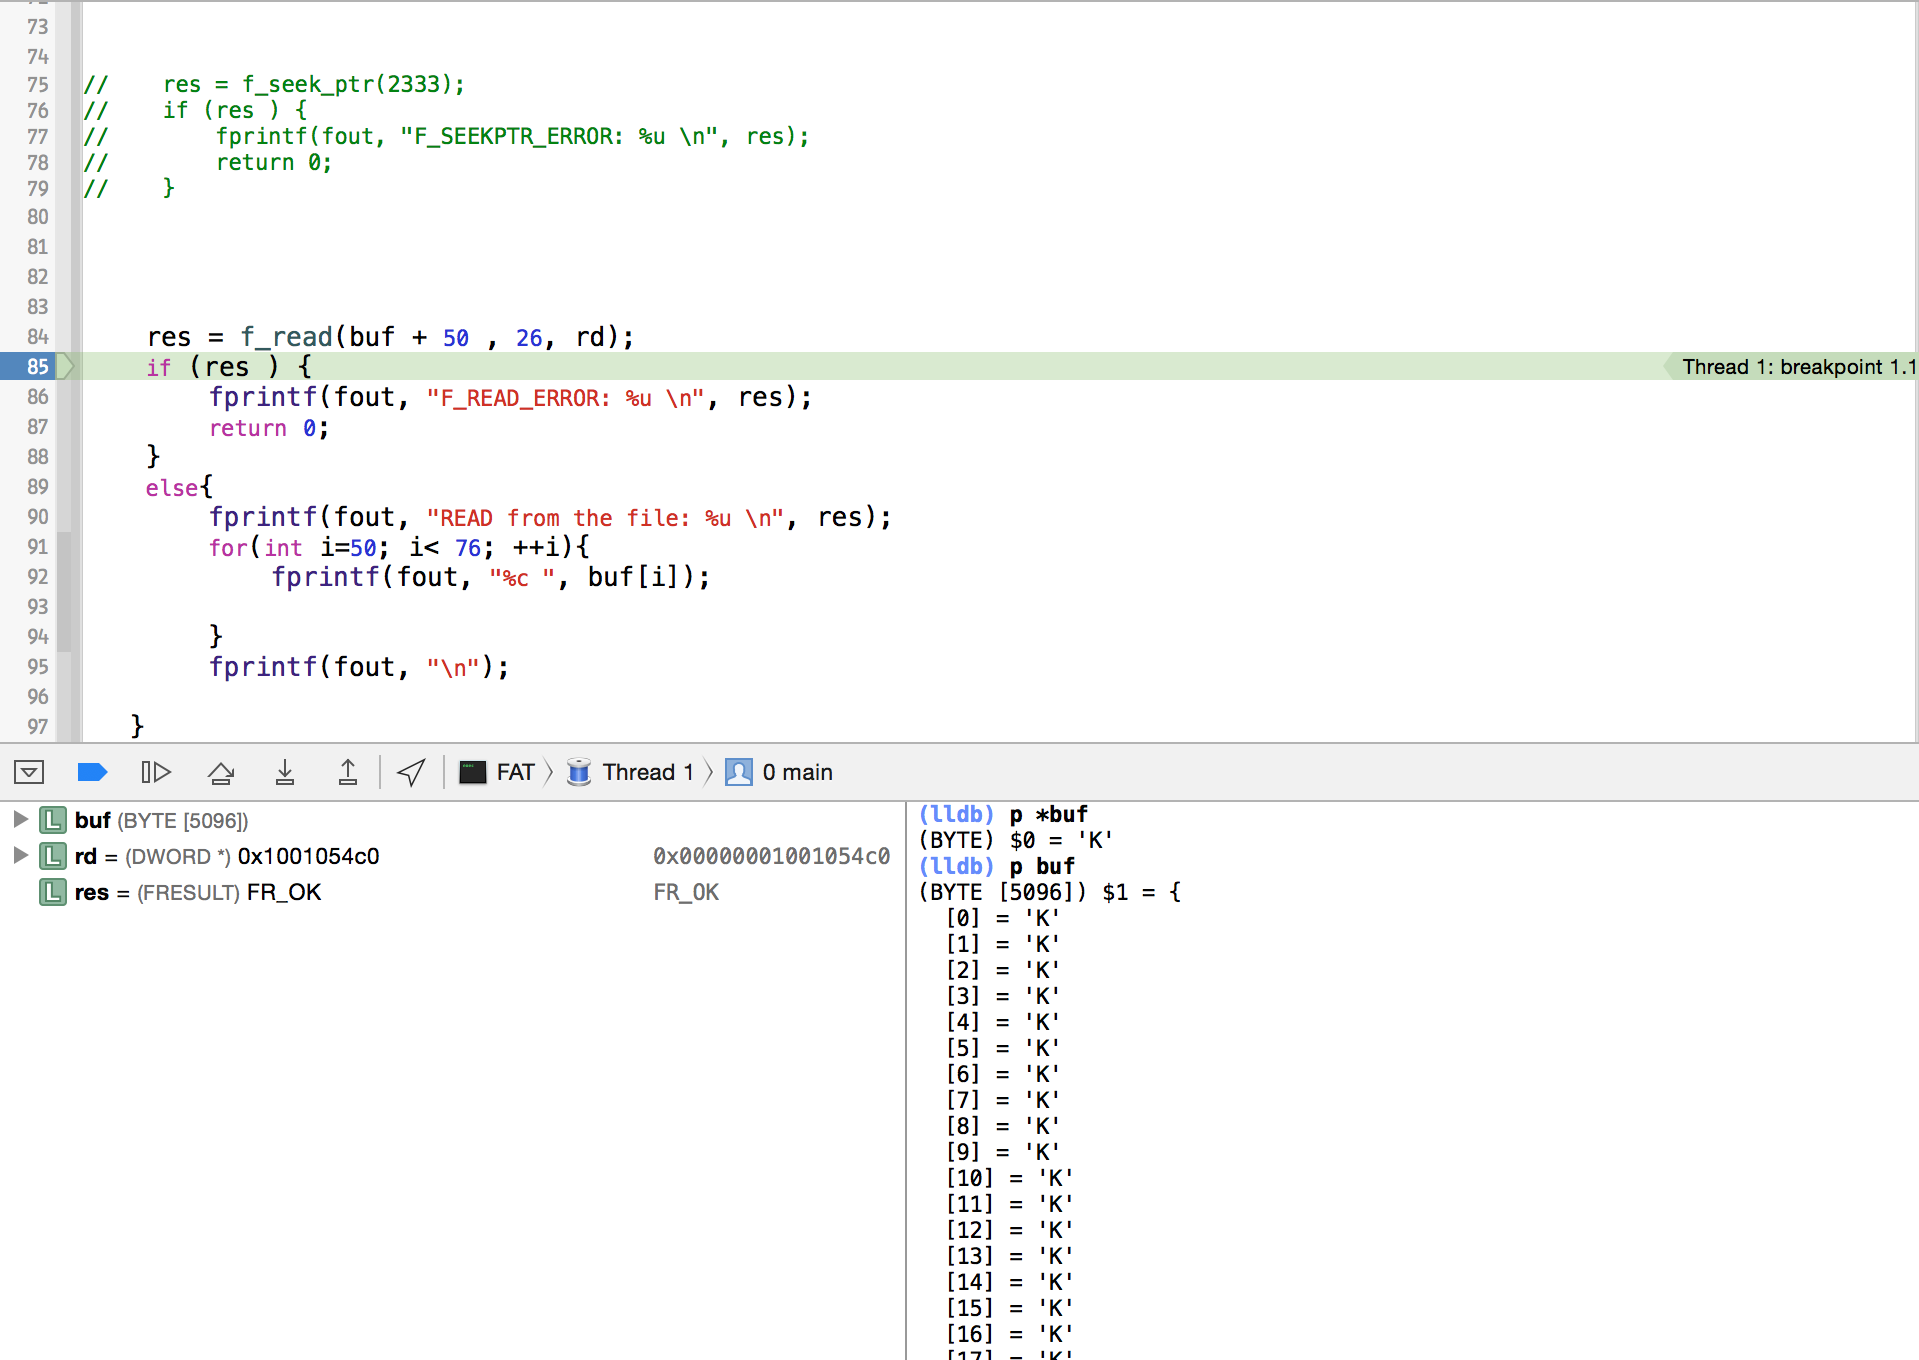
\includegraphics[width=1.0\linewidth]{chap4/datard.png}
    \\
    \caption{读文件的结果} \label{fig:datard}
\end{figure}

最后的实验项目是删除文件,删除文件不仅要删除目录表的记录,还要清除FAT表的相应簇链。
删除后结果如图\ref{fig:dirrm}和\ref{fig:fatrm}。

\begin{figure}[!htbp]
    \centering
    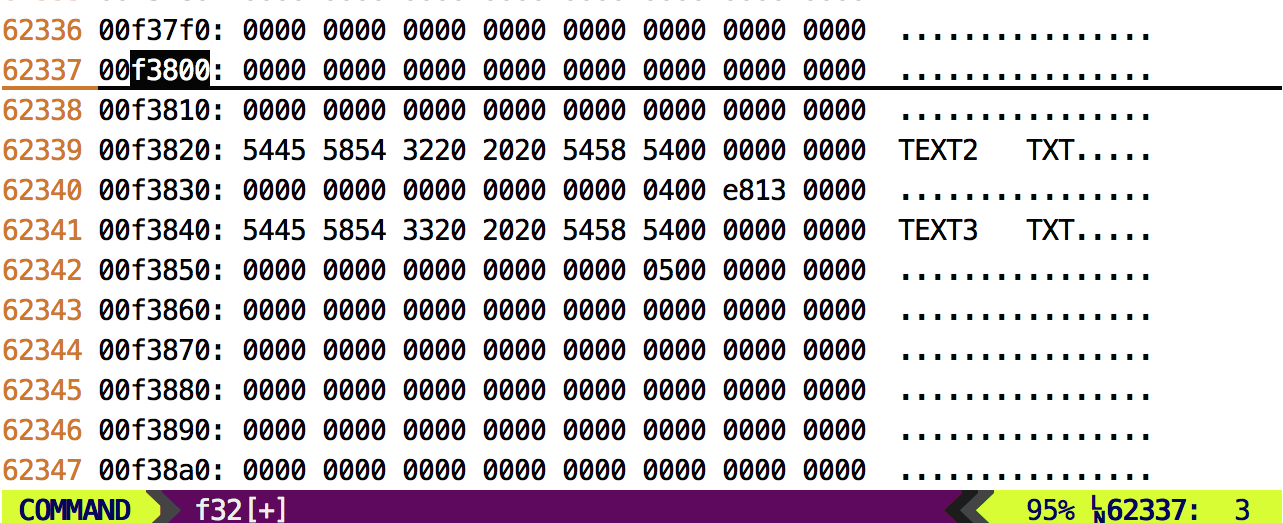
\includegraphics[width=1.0\linewidth]{chap4/dirrm.png}
    \\
    \caption{删除后的目录表} \label{fig:dirrm}
\end{figure}

\begin{figure}[!htbp]
    \centering
    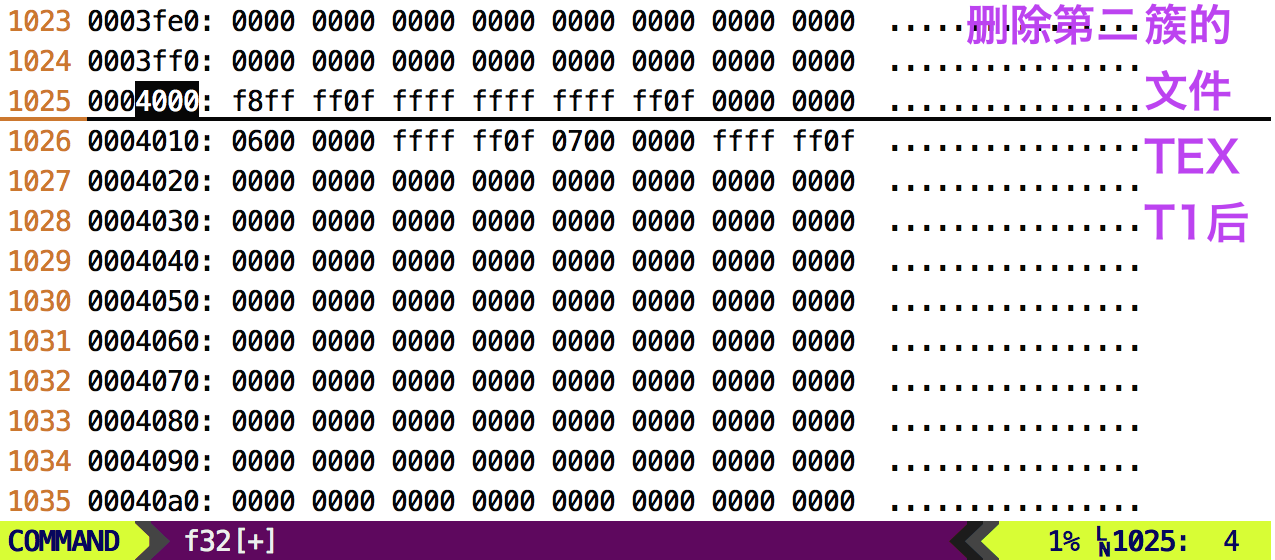
\includegraphics[width=1.0\linewidth]{chap4/fatrm.png}
    \\
    \caption{删除后的FAT表} \label{fig:fatrm}
\end{figure}

\section{实际的实验验证}
\label{sec:ExpDriver}
整个文件接口的实现过程必须和底层的硬件相契合,对于不同的硬件或者不同的环境,都要求做出相应的调整。
本工程实现过程中用到了以C8051F020为MCU的单片机,同时用到了一个SD卡槽,该卡槽是11脚卡槽。

实验测试的SD卡是一张4GB的SDHC卡,实际上本接口能够支持几乎所有类型的SD卡,即使是老版本(Version 1.x)的老式卡也没有问题。
实验用到的板子如图\ref{fig:mcu}和\ref{fig:11sd}所示。鉴于本实验只需使用C8051F020的「P0.0」-「P0.3」引脚,再加一根片选线「CS」,本实验将其分配给了「P3.1」。
硬件SPI的「P0.3」是「NSS」位,是输入信号,只做从机片选,不能用做CS输出片选,因此要将它始终拉高(不使能)。

由于微处理器所在的板子没有SD卡槽,故另外引了4根数据线到图\ref{fig:11sd}中的SD卡槽。
该11脚的SD卡槽,
比正常的9脚SD卡多了两个保护引脚,其中一个保护引脚是卡插入检测位「CD」,
然而该引脚并没有接在SD卡的「CD/DAT3」引脚上。对于11脚的卡槽,「DAT3」脚与SD卡的「CD/DAT3」相连接。
在程序运行中,本接口通过判断「CD」引脚的电平高低来进行SD卡的插入拔出检测,当SD卡正确插入后,「CD」被拉低,否则其始终为高电平。

\begin{figure}[!htbp]
    \centering
    \includegraphics[width=1.0\linewidth]{chap4/mcu.png}
    \\
    \caption{C8051F020} \label{fig:mcu}
\end{figure}

\begin{figure}[!htbp]
    \centering
    \includegraphics[width=1.0\linewidth]{chap4/11sd.png}
    \\
    \caption{SD卡槽} \label{fig:11sd}
\end{figure}

整体的实验环境如图\ref{fig:vol}

\begin{figure}[!htbp]
    \centering
    \includegraphics[width=1.0\linewidth]{chap4/vol.png}
    \\
    \caption{硬件环境} \label{fig:vol}
\end{figure}

在SD卡中新建「TEXT6.TXT」等文件后,将SD插入PC机,可以识别。
并且「TEXT6.TXT」文件被写入了37KB的数据用来测试跨簇大文件的支持程度,而「TEXT1.TXT」仅写入了4KB数据,
「TEXT10.TXT」是新创建的文件,还没有写入数据。

\begin{figure}[!htbp]
    \centering
    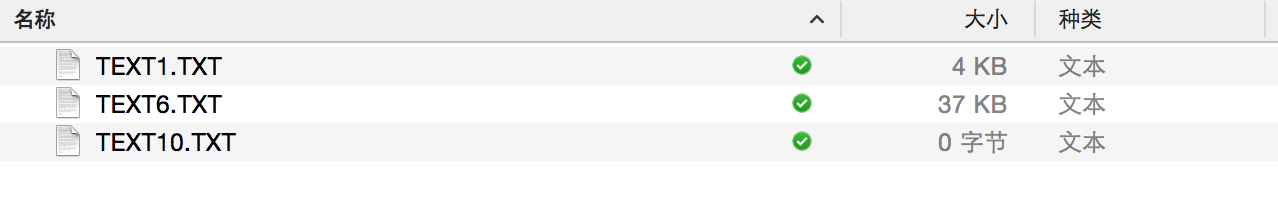
\includegraphics[width=1.0\linewidth]{chap4/sdwrt.png}
    \\
    \caption{SD卡插入PC后} \label{fig:sdwrt}
\end{figure}

为了测试大文件写入过程是否顺利,但是单片机有没有足够大的内存空间,故选择了使用同一个缓冲池循环写入。同时为了快速更换缓冲池的内容,
直接通过「memset()」函数对其赋值。

\begin{figure}[!htbp]
    \centering
    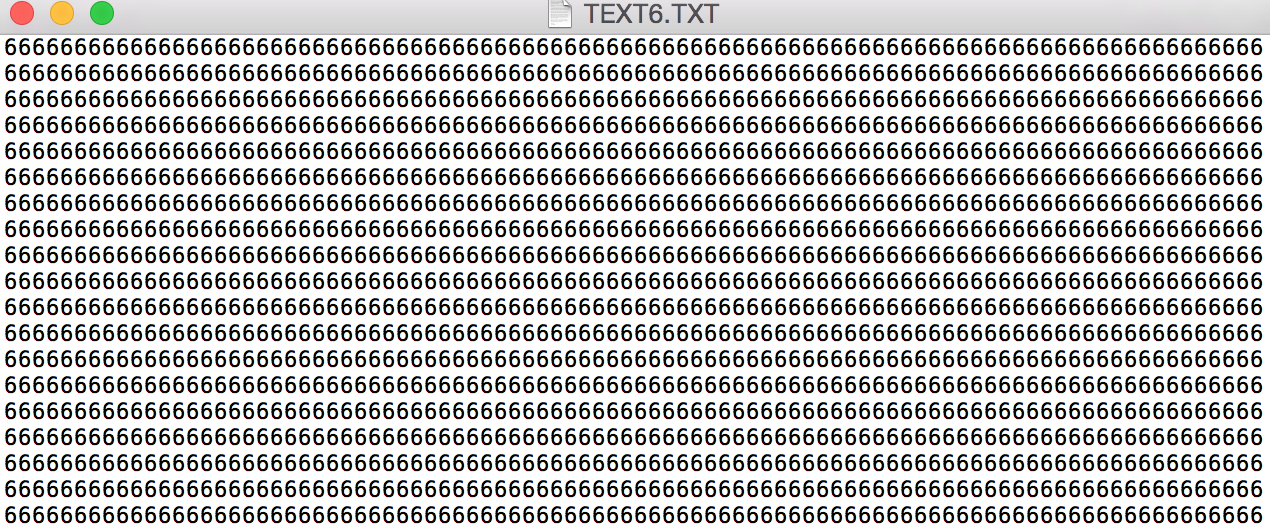
\includegraphics[width=1.0\linewidth]{chap4/sddata.png}
    \\
    \caption{写入长数据后文件的内容} \label{fig:sddata}
\end{figure}

可以看到,计算机是能该正确读取单片机向SD卡的文件中写入的数据的。

\section{结果}
\label{sec:Conclusion}
通过本次的实验和验证,成功完成了本FAT32文件接口对以SD卡为介质的文件系统的操作。
单片机通过本文件接口,实现了对FAT文件系统的挂载,能够在根目录新建文件和删除文件,
并且能够打开文件进行读写操作,跨簇的大文件长文件也完全没有问题。

预期的要实现的目标包括文件系统挂载、SD卡插拔检测、文件的新建与删除、打开关闭文件及读写文件等功能均能够顺利实现,
并且本接口还能够在文件的特定位置读写文件。

上述的各项操作都是以FAT32文件系统的规范为标准,完全契合并兼容FAT32文件系统,使得计算机在插入SD卡后,能够浏览根目录下的单片机所创建的各项文件,
并且也能够正确识别并打开这些文件进行读取和修改,这使得单片机与计算机的协同工作能力得到极大的提升,二者的联系更为密切,
它们之间进行数据共享可以通过SD卡方便的完成。

\section{小结}
\label{sec:Sum4}
本章详细描述了具体的实验过程及实验验证结果,首先进行上层FAT模块的逻辑实验验证,仅验证测试其逻辑功能。然后,当模块化测试通过后,
在使之与底层的SD卡驱动模块结合起来进行联合调试,在具体的实际操作中进行实验验证。
最终结果显示整个文件接口符合要求,各预期功能顺利达成。
